%\section{Voice Commands}
\section{Design Goals}
\label{sec:motivation}

\begin{figure}[t]
    \centering
    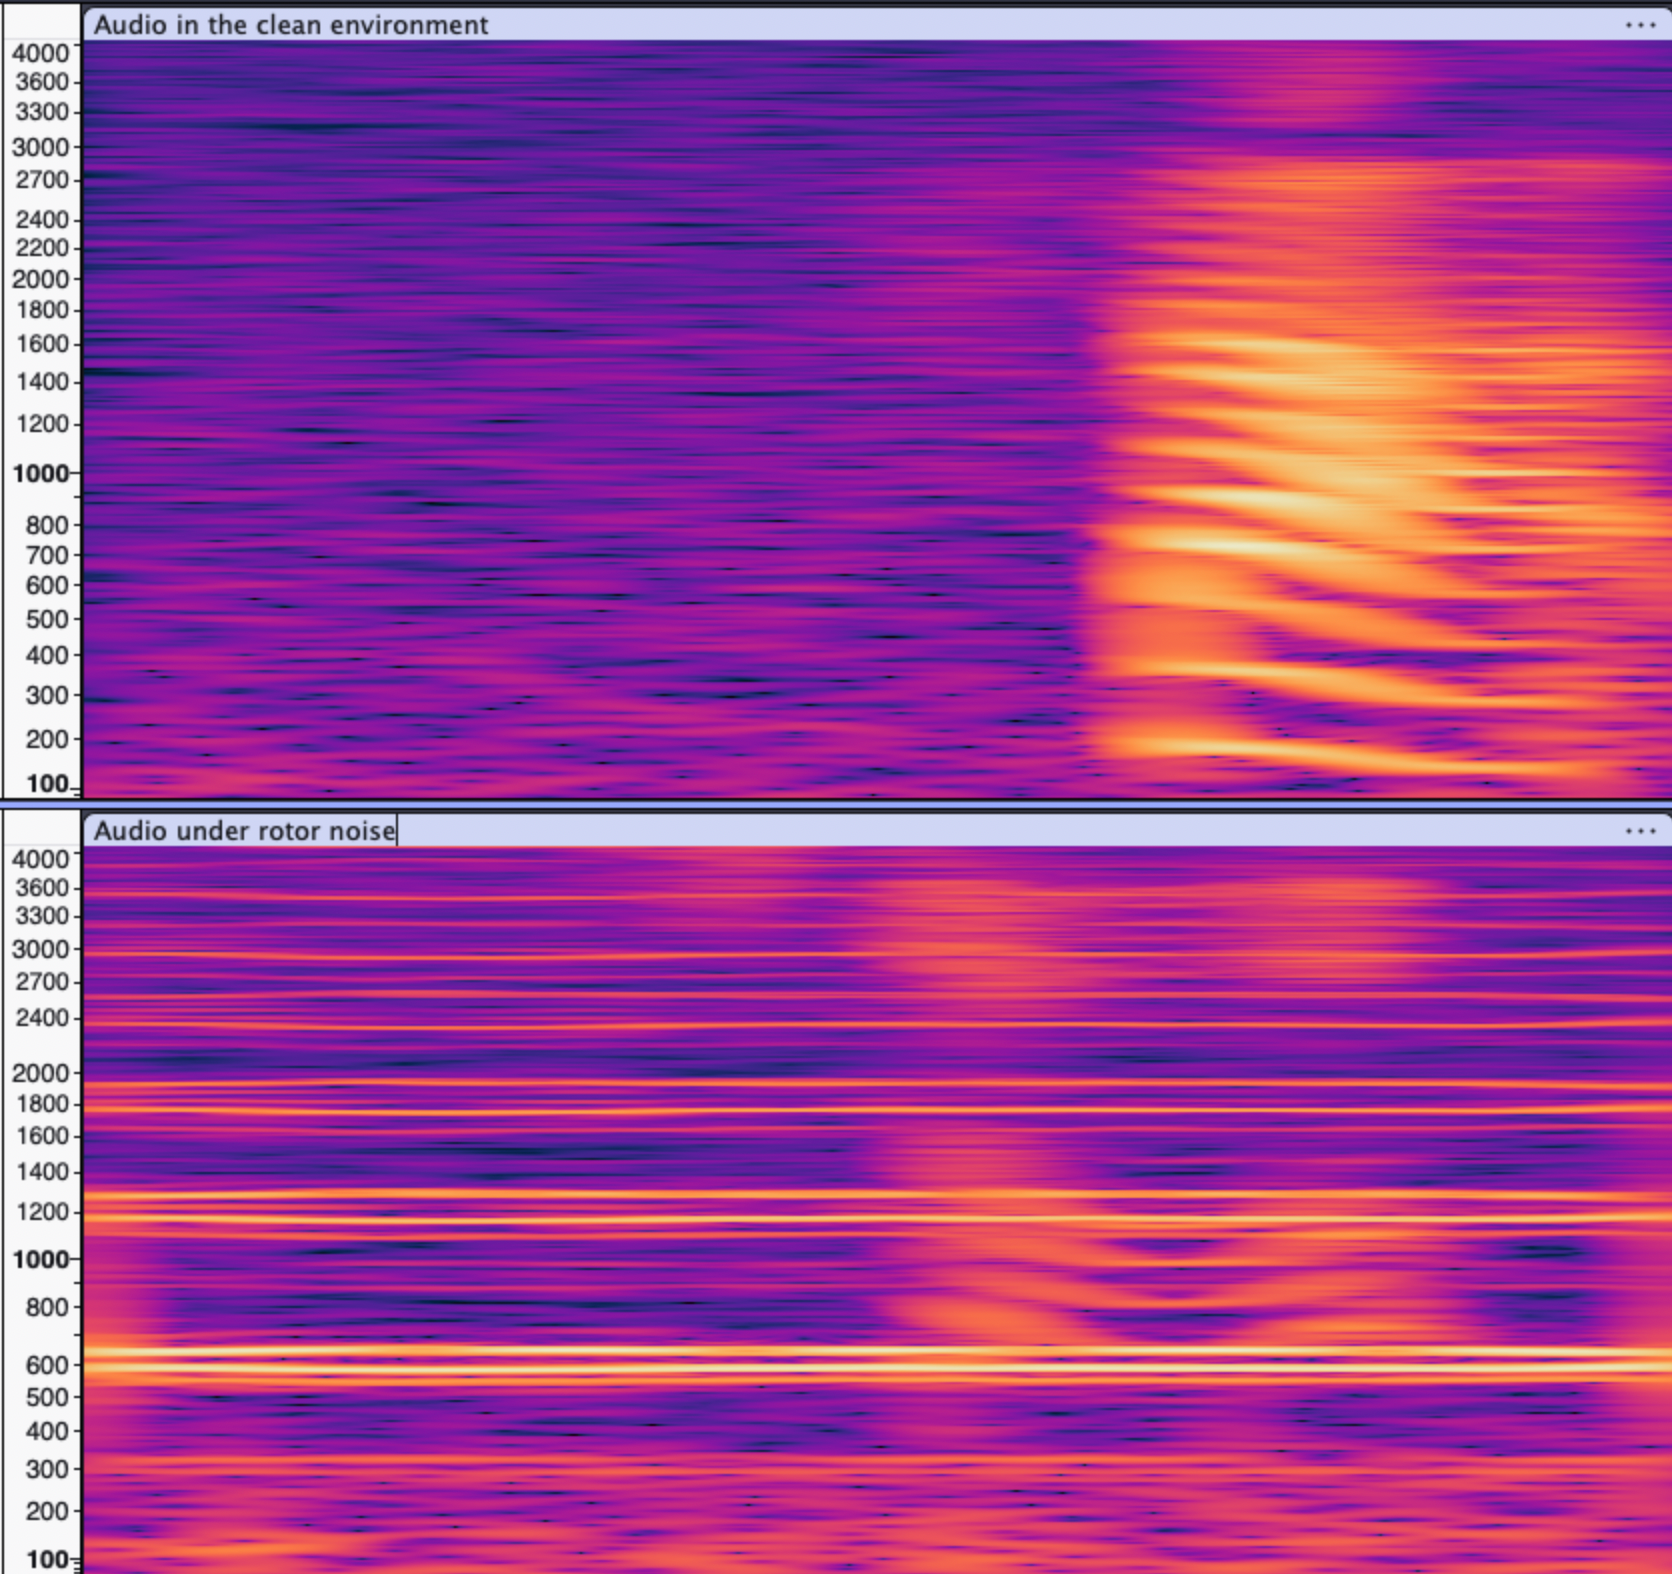
\includegraphics[width=\columnwidth, height=0.4\linewidth]{figures/cleanvsnoisy.png}
    \caption{Clean versus rotor-noisy log-mel. The example illustrates why nearby UAV speech differs quite from usual command recognition Apps, which are handheld and away from UAVs.}
    \label{fig:clean_vs_noisy}
    \vspace{-15pt}
\end{figure}

\subsection{Voice Input for Physical Risk Aversion}
Voice is a natural way for people to interact with a nearby drone because it does not require opening an application, finding a controller, or relying on commands through an application via a supporting network. This matters most when the interaction is time-sensitive: a person may need to ask the drone to stop, hold position, or respond to a safety-critical situation. At the same time, the UAV is already close to people or objects. The design goal is not to replace existing UAV safety mechanisms. It is to add an audio substrate that can expose the nearby human intent to control UAVs. 

The difficulty is that a voice interface near a UAV is not only a speech-recognition problem. Speech is ambiguous, background audio is uncontrolled, and the drone itself creates rotor self-noise. A wrong speech decision can also have a physical interpretation--a missed emergency can delay a safety response, while a false movement or emergency trigger can interrupt the UAV at the wrong time. Work on always-on and embedded speech systems already shows that false accepts, misses, latency, and runtime constraints matter in addition to top-line accuracy \cite{rybakov2020streamingkws,banbury2021mlperftiny}. For a UAV, those errors must be mediated before they reach the control stack.

This is why the voice layer must remain conservative. The system should not treat a noisy utterance as a direct command, even when the recognizer is accurate on average. The useful output of speech recognition is evidence for a downstream safety decision: an intent-state update that can be logged, ignored, held, escalated, or forwarded by a safety-state boundary.

This role complements existing UAV safety mechanisms rather than replacing them. Obstacle-avoidance sensors detect nearby objects but not a person's spoken intent. Geofencing constrains where the UAV may operate, but does not capture local human requests. Failsafe landing responds to UAV or link failures, while nearby speech can surface safety-critical concerns before such a failure state is reached. Manual controllers provide explicit control, but require device access. \sys{} adds a hands-free speech channel whose output remains mediated by the safety-state boundary.

\subsection{Failure Modes of Common Speech Interfaces}

The most direct design is a transcript-first pipeline: run speech-to-text, then parse the transcript for command words. This is attractive because it appears general and easy to extend. The problem is that nearby UAV audio is short, noisy, and action-sensitive. Rotor self-noise can reduce transcript coverage in one-second clips, and an incomplete or distorted transcript can make the parser miss an emergency phrase or extract the wrong command. This is a scoped concern about short rotor-noisy clips, not a universal statement about every ASR configuration; longer context, different microphones, or larger models may improve transcript quality. The system hazard is that transcript-first processing asks the system to recover free-form text even though the control side needs only a narrow, safety-relevant decision.

Keyword spotting and compact speech-command classifiers avoid full transcripts and are much closer to embedded deployment \cite{sainath2015cnn_kws,warden2018speechcommands,zhang2017helloedge}. They are useful baselines for limited-vocabulary recognition, but a detected keyword or command class is still not a safety mechanism. A keyword trigger does not say whether a movement request has authority, whether the UAV state permits action, whether an emergency-like word should interrupt the current task, or whether repeated detections should be suppressed. Without a safety-state boundary, the classifier output can become a direct trigger rather than a controlled input.

Direct speech-to-command mapping creates the sharpest hazard. If every recognized emergency or movement label is bound to an action, then recognition errors become action pressure on the control stack. False emergency predictions can create unnecessary interruptions, false movement predictions can request unauthorized motion, and missed emergency speech can leave the voice channel silent when it is needed. This is a design hazard that follows from binding noisy recognition output directly to action.

Removing the unknown fallback creates a related failure mode. Unsupported speech, background audio, or low-confidence windows still have to go somewhere. If the classifier has only actionable classes, then unsupported audio is forced into emergency or movement. For a UAV, that forced decision is not just a classification error. It is pressure on the safety-state boundary to handle audio that should have remained non-actionable.

\subsection{Constrained Intent-State Updates}

Small drones create their own acoustic interference. The microphone is close to the rotors, the noise changes with operating state, and the resulting speech condition differs from quiet indoor command recognition. Prior UAV speech-interface and UAV-noise studies motivate this setting \cite{oneata19_interspeech,oneata2021multimodal,miesikowska2021uavnoise,park2023uavUAV}, and broader drone-audition work treats platform ego-noise as a core obstacle for aerial audio sensing \cite{chevtchenko2025drone_ssl}. The clean-versus-noisy example in Figure~\ref{fig:clean_vs_noisy} illustrates the kind of acoustic shift that the system must handle.

The design response is to make speech produce constrained intent-state updates, not transcripts or direct commands. The paper uses a deliberately narrow intent-state mapping: \emph{emergency}, \emph{movement}, and \emph{unknown}. Emergency represents safety-critical speech that can be handled differently by the safety-state boundary. Movement represents ordinary control-oriented speech, but it remains pending until downstream safety logic supplies direction, authorization, and UAV-state checks. Unknown represents unsupported or uncertain audio. This mapping is the reason the recognizer can participate in a safety layer: it prevents every utterance from being forced into an actionable command class.

The same safety motivation also argues for local inference. A voice safety layer should remain available when a phone application is not open, a network path is unreliable, or a cloud service would add an avoidable dependency. Local deployment turns recognition into a systems problem: the model must fit the embedded operator set and memory budget, report timing and confidence, and expose enough state for the safety-state boundary to audit the decision. Microcontroller speech runtimes and benchmarks make this constraint explicit by treating kernels, memory, latency, energy, and target hardware as part of the result \cite{david2021tflm,lai2018cmsisnn,banbury2021mlperftiny}. The required output is therefore a local intent-state update stream with confidence and timing, followed by boundary checks that decide whether to ignore, hold, escalate, or forward the update.
